\chapter{\textbf{Аналитический раздел}}
\hfill

Целью данной работы является реализация загружаемого модуля ядра для отслеживания USB­-устройств, являющихся ключом для доступа к приложению. В данном разделе производится постановка задачи и рассмотрение основных понятий. 

\section{\textbf{Постановка задачи}}

Требуется разработать программное обеспечение для отслеживания USB­-устройств, который обладает следующей функциональностью:
\begin{itemize}
\item список разрешенных устройств;
\item список путей к секретным файлам;
\item отслеживание появления новых USB­-устройств;
\begin{itemize}
\item если устройство известно, происходит расшифровка файла;
\item если устройство не известно, происходит зашифровка файла. 
\end{itemize}
\end{itemize}

На вход подается USB устройство с паролем. На выходе получаем зашифрованный или расшифрованный файл.

\section{\textbf{Загружаемый модуль ядра}}

Ядро Linux динамически изменяемое -- это означает, что вы можете загружать в ядро дополнительную функциональность, выгружать функции из ядра и даже добавлять новые модули, использующие другие модули ядра. Преимущество загружаемых модулей заключается в возможности сократить расход памяти для ядра, загружая только необходимые модули (это может оказаться важным для встроенных систем).

Загружаемый модуль представляет собой специальный объектный файл в формате ELF (Executable and Linkable Format). Обычно объектные файлы обрабатываются компоновщиком, который разрешает символы и формирует исполняемый файл. Однако в связи с тем, что загружаемый модуль не может разрешить символы до загрузки в ядро, он остается ELF-объектом. Для работы с загружаемыми модулями можно использовать стандартные средства работы с объектными файлами (имеют суффикс .ko, от kernel object). \cite{kernelmodules}


В OC Linux существуют специальные команды для работы с загружаемыми модулями ядра.

insmod -- Загружает модуль в ядро из конкретного файла, если модуль зависит от других модулей. Только суперпользователь может загрузить модуль в ядро.

lsmod -- Выводит список модулей, загруженных в ядро.

modinfo -- Извлекает информацию из модулей ядра (лицензия, автор, описание и т.д.).

rmmod -- Команда используется для выгрузки модуля из ядра, в качестве параметра передается имя файла модуля. Только суперпользователь может выгрузить модуль из ядра.

Загружаемые модули ядра должны содержать два макроса module\_init и module\_exit.

\section{\textbf{Уведомления в ядре Linux}}

\subsection{\textbf{Уведомители}}

Ядро Linux содержит механизм, называемый <<уведомителями>> (notifiers) или <<цепочками уведомлений>> (notifiers chains), который позволяет различным подсистемам подписываться на асинхронные события от других подсистем. Цепочки уведомлений в настоящее время активно используется в ядре; существуют цепочки для событий hotplug памяти, изменения политики частоты процессора, события USB hotplug, загрузка и выгрузка модулей, перезагрузки системы, изменения сетевых устройств и т. д. \cite{notifications}

Основной является структура notifier\_block, листинг которой представлен в \ref{lst:notifier_block}.

 \begin{lstlisting}[caption = Структура notifier\_block, label =  lst:notifier_block]
 struct notifier_block {
    notifier_fn_t notifier_call;
    struct notifier_block __rcu *next;
    int priority;
 };
 \end{lstlisting}
 
Структура определен в \#include/linux/notifier.h. Эта структура содержит указатель на функцию обратного -- notifier\_call, ссылку на следующий notifier\_block и приоритет функции, функции с более высоким приоритетом выполняются первыми.

\subsection{\textbf{Уведомитель изменений на USB портах}}

Существует уведомитель, позволяющий отслеживать изменения на usb портах. \cite{usbnotifications}

\textit{void usb\_register\_notify(struct notifier\_block *nb);}

\textit{void usb\_unregister\_notify(struct notifier\_block *nb);}

Существующие события: \textit{USB\_DEVICE\_ADD} -- добавление нового устройства, \textit{USB\_DEVICE\_REMOVE} -- удаление устройства.

\section{\textbf{Хранение информации о доступных USB устройствах}}

Для хранения устройств будет использовать двусвязный список ядра Linux, реализованный в файле \#include/linux/list.h. \cite{lists}

\textit{LIST\_HEAD} -- объявление и инициализация головы списка.

\textit{list\_for\_each\_entry(temp, \&connected\_devices, list\_node)} -- проход по списку.

\textit{list\_for\_each\_entry\_safe(device, temp, \&connected\_devices, list\_node)} -- «защищенный» проход по всем элементам списка, используется для удаления записей списка.

\textit{list\_add\_tail(struct list\_head * new, struct list\_head * head) }-- добавление нового элемента.

\section{\textbf{Вызов приложений пользовательского пространства из ядра}}

Usermode-helper API -- это простой API с известным набором опций. Например, чтобы создать процесс из пользовательского пространства, обычно необходимо указать имя исполняемого файла, параметры исполняемого файла и набор переменных среды. \cite{userspace}

\textit{int call\_usermodehelper(const char *path, char **argv, char **envp, int wait)} -- подготовить и запустить приложение пользовательского режима.

\textit{const char * path} -- путь к исполняемому файлц пользовательского режима.

\textit{char ** argv} -- параметры.

\textit{char ** envp} --  переменные среды.

\textit{int wait}  -- дождитесь завершения работы приложения и возврата статуса.

Реализация usermodehelper проста и понятна, рисунок \ref{img:user_kernel}.

\textit{UMH\_WAIT\_PROC} -- если запрашивающий хочет дождаться завершения всего процесса, включая вызов пользовательского пространства, \textit{UMH\_NO\_WAIT} -- вообще не ждать, \textit{UMH\_WAIT\_EXEC} -- дождаться вызова приложения пользовательского пространства, но не завершения.

\begin{figure}[H]
	\centering
	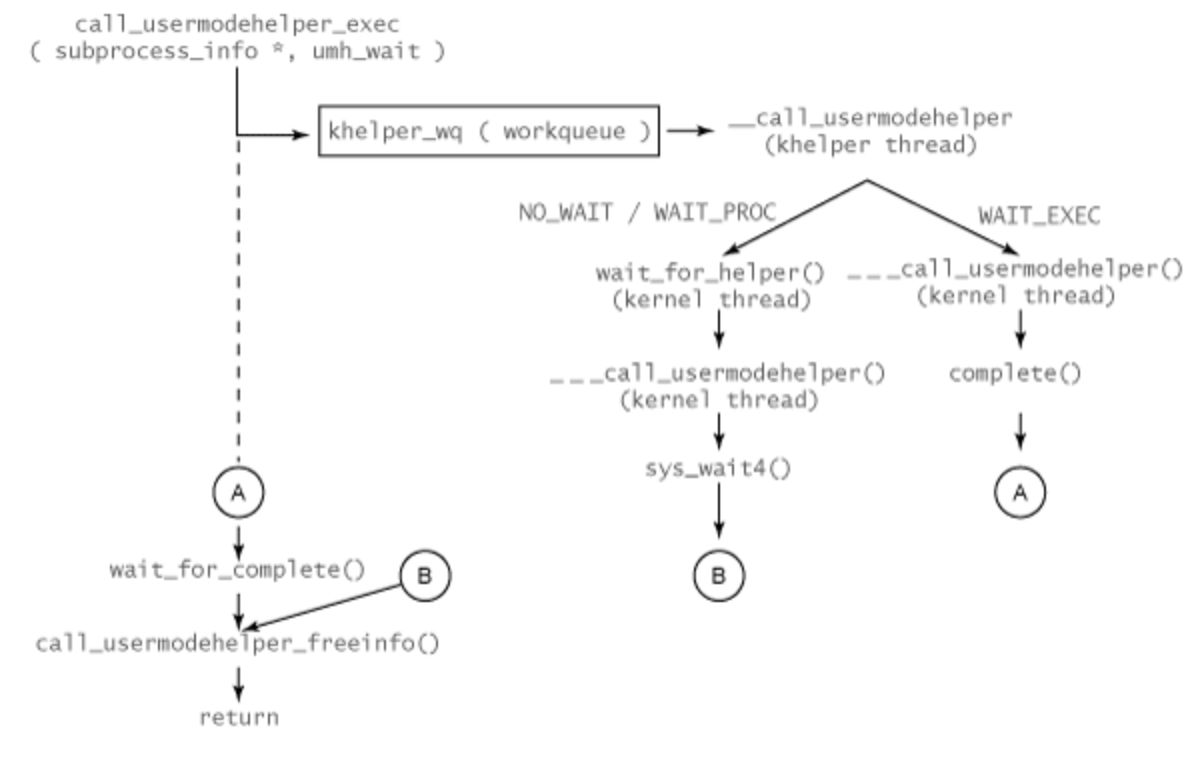
\includegraphics[scale=0.8]{user_kernel}
	\caption{Внутренняя реализация API usermodehelper. }
	\label{img:user_kernel}
\end{figure}

\section{\textbf{Чтение и запись файлов в пространстве ядра}}

Иногда необходимо читать и записывать файловые данные в ядре Linux. \cite{read_write}

В основном это функции: 

\textit{struсt file* filp\_open(const char* filename, int open\_mode, int mode)} -- открытие файла в ядре. filename -- имя файла, который может быть создан или открыт, включает путь до файла; open\_mode -- режим открытия файла O\_CREAT, O\_RDWR, O\_RDONLY, mode -- используется при создании файла, установите разрешения на чтение и запись созданного файла, в противном случае он может быть установлен в 0.

\textit{int filp\_close(struct file*filp, fl\_owner\_t id)} -- закрытие файла.
 
\textit{ssize\_t vfs\_read(struct file* filp, char \_\_user* buffer, size\_t len, loff\_t* pos)}, \textit{ssize\_t vfs\_write(struct file* filp, const char \_\_user* buffer, size\_t len, loff\_t* pos)} -- чтение и запись файлов в ядре.

Второй параметр этих двух функций имеет перед собой модификатор \_\_user, который требует, чтобы оба указателя буфера указывали на память пространства пользователя. Чтобы эти две функции чтения и записи правильно работали с указателем буфера в пространстве ядра, вам нужно использовать функцию set\_fs(). Ее функция состоит в том, чтобы изменить способ, которым ядро обрабатывает проверку адресов памяти. На самом деле параметр fs этой функции имеет только два значения: USER\_DS и KERNEL\_DS, которые представляют пространство пользователя и пространство ядра соответственно.

\textit{void set\_fs(mm\_segment\_t fs)}

\textit{mm\_segment\_t  get\_fs ()}

\section{\textbf{Основные используемые структуры}}

В данной работе происходит отслеживание изменений на usb портах, основными структурами являются usb\_device и usb\_device\_id.

\subsection{\textbf{usb\_device}}

Структура usb\_device приведена в листинге \ref{lst:usb_device} -- представление USB-устройста в ядре.

Используемые поля:

descriptor -- дескриптор USB устройства. 

Каждое продающееся устройство с USB требует сертификации на соответствие требованиям USB, для чего ему необходимо иметь ID поставщика (vendor ID) и ID изделия (product ID). Эти поля присутствуют в descriptor, используются для идентификации USB устройства. 

\subsection{\textbf{usb\_device\_id}}

Структура usb\_device\_id приведена в листинге \ref{lst:usb_device_id} -- идентификация USB устройств для отслеживания и подключения.

Используемые поля:

idVendor -- ID поставщика; 

idProduct -- ID изделия.

\section{\textbf{Вывод}}

В данном разделе была постановлена задача и рассмотрены основные понятия. 